\chapter{SYSTEM ARCHITECTURE}

\section{Block Diagram}
This chapter describes the pictorial representation of the process flow in the development of the product. The block diagram illustrates the end-to-end communication from the BLE Tag to the Admin Dashboard. 

\begin{figure}[H]
\centering
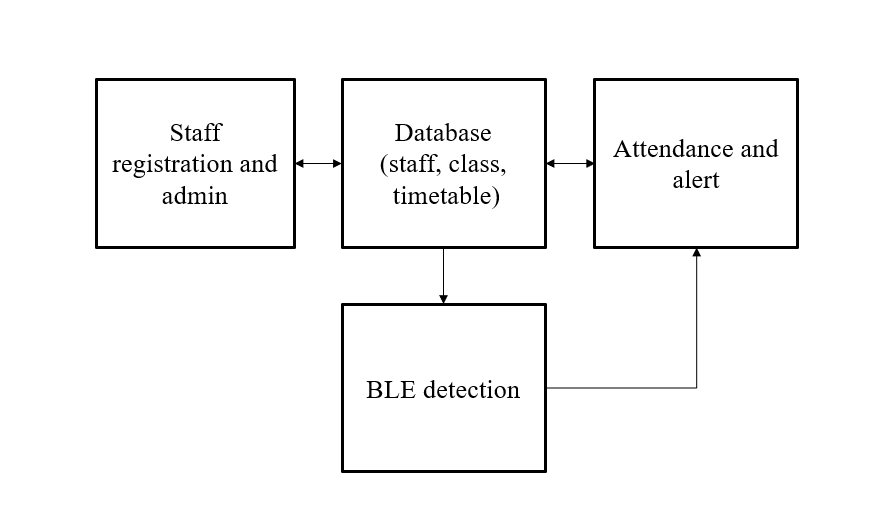
\includegraphics[width=0.8\textwidth]{images/block_diagram.png}
\caption{System Block Diagram}
\end{figure}

\section{Presence Verification Workflow}
The presence verification process is based on a context-aware approach. The system verifies two important factors: location and time. The location is determined using the BLE signal detected by the ESP32 receiver placed in the classroom. The time is verified using the timetable stored in the database. 

\section{Data Dictionary (Database Design)}
The following tables represent the technical schema of the MongoDB collections used in the Staff Presence Verification system. 

\subsection{Staff Collection}
\begin{table}[H]
\centering
\caption{Staff Table Schema}
\begin{tabular}{|p{3cm}|p{3cm}|c|p{4cm}|}
\hline
\textbf{Field Name} & \textbf{Data Type} & \textbf{Key} & \textbf{Description} \\ \hline
\_id & ObjectId & PK & Unique identifier for the staff. \cr \hline
name & String & - & Full name of the staff member. \cr \hline
beacon\_uuid & String & Unique & Unique BLE tag identifier. \cr \hline
department & String & - & Academic department. \cr \hline
designation & String & - & Position (Professor/AP). \cr \hline
\end{tabular}
\end{table}

\subsection{Timetable Collection}
\begin{table}[H]
\centering
\caption{Timetable Table Schema}
\begin{tabular}{|p{3cm}|p{3cm}|c|p{4cm}|}
\hline
\textbf{Field Name} & \textbf{Data Type} & \textbf{Key} & \textbf{Description} \\ \hline
staff\_id & ObjectId & FK & Reference to Staff collection. \cr \hline
classroom\_id & ObjectId & FK & Reference to Classroom. \cr \hline
day\_of\_week & String & - & Weekday name. \cr \hline
start\_time & String & - & Opening period time. \cr \hline
end\_time & String & - & Closing period time. \cr \hline
\end{tabular}
\end{table}

\subsection{Attendance Collection}
\begin{table}[H]
\centering
\caption{Attendance Table Schema}
\begin{tabular}{|p{3cm}|p{3cm}|c|p{4cm}|}
\hline
\textbf{Field Name} & \textbf{Data Type} & \textbf{Key} & \textbf{Description} \\ \hline
staff\_id & ObjectId & FK & Staff reference. \cr \hline
date & Date & - & Day of logging. \cr \hline
status & String & - & Present/Absent/Late log. \cr \hline
check\_in & Date & - & Logged presence start. \cr \hline
\end{tabular}
\end{table}

\section{Hardware and Communication Module}
The ESP32 receiver acts as the primary hardware gateway. It uses dual-mode BLE scanning to detect both generic iBeacons and mobile devices configured for Bluetooth advertising. 
